\section{Filtered-x Least mean square}


\subsection{The general system}
\begin{frame}{Filtered-$x$ Least mean squares}{The General System}
	\begin{columns}
		\begin{column}{0.5\textwidth}		

		\begin{itemize}
		\item Feedforward
		\begin{itemize}
		\item Dependent on delay between actuator and source		
		\end{itemize}
		\item Combined with an error microphone for feedback
		\begin{itemize}
		\item Adapt to changes in environment
		\item Always behind in samples/time 		
		\begin{itemize}
		\item Efficient for periodic signals
		\item Inefficient for stochastic signal 
		\end{itemize}	
		\end{itemize}
		\item Assumptions:
		\begin{itemize}
		\item Stationary Cancellation path
		\item FIR filter
		\end{itemize}

		\end{itemize}

		
		\end{column}
		\begin{column}{0.5\textwidth}
		\resizebox{1.1\columnwidth}{!}{	
		\begin{tikzpicture}
\draw [](-2.92,2.32) node (v1) {} .. controls (-3.26,2.06) and (-3.26,0.54) .. (-2.92,0.32) node (v2) {};

\draw [draw=black,fill=black!20](-0.68,2.32) node (v1) {} .. controls (-1.08,2.06) and (-1.08,0.54) .. (-0.68,0.32) node (v2) {};
\draw [white, fill=black!20](-0.68,2.32) -- (1.56,2.32) -- (1.56,0.32) -- (-0.68,0.32);


\draw [draw=black,fill=black!60](-0.93,1.78) node (v1) {} .. controls (-0.99,1.59) and (-0.99,1.14) .. (-0.95,0.94) node (v2) {};
\draw [draw=black,fill=black!60](-0.93,1.78) -- (0.72,1.78) -- (0.72,0.94) -- (-0.95,0.94);


\draw [draw=black,fill=white] (0.48,1.36) node (v3) {3} ellipse (0.2 and 0.3);
\draw [draw=black,fill=black](0.28,1.66) -- (0.28,1.06);

\draw [draw=black,fill=white] (-3.4,1.36) node (v3) {1} ellipse (0.2 and 0.3);
\draw [draw=black,fill=black](-3.6,1.7) -- (-3.6,1.06);


\draw [draw=black,fill=black] (-2.9,1.7) rectangle (-3,1);
\draw (-2.9,1.3) -- (-2.6,1.7) -- (-2.6,1) -- (-2.9,1.3);
\node at (-2.7,1.34) {\small{2}};
\node at (-1.7,1.54) {\small{c[n]}};

\draw[->,dashed] (-2.6,1.36) node[right=0.5,above]{\small{}}-- (0.28,1.36);



\draw [->](-1.14,-1.76) -- (-1.14,-0.2) -- (-2.94,-0.2) -- (-2.94,1);
\node at (0,2) {\small{Ear Canal}};
\node[anchor=south west,inner sep=0] at (1.9,0.3) {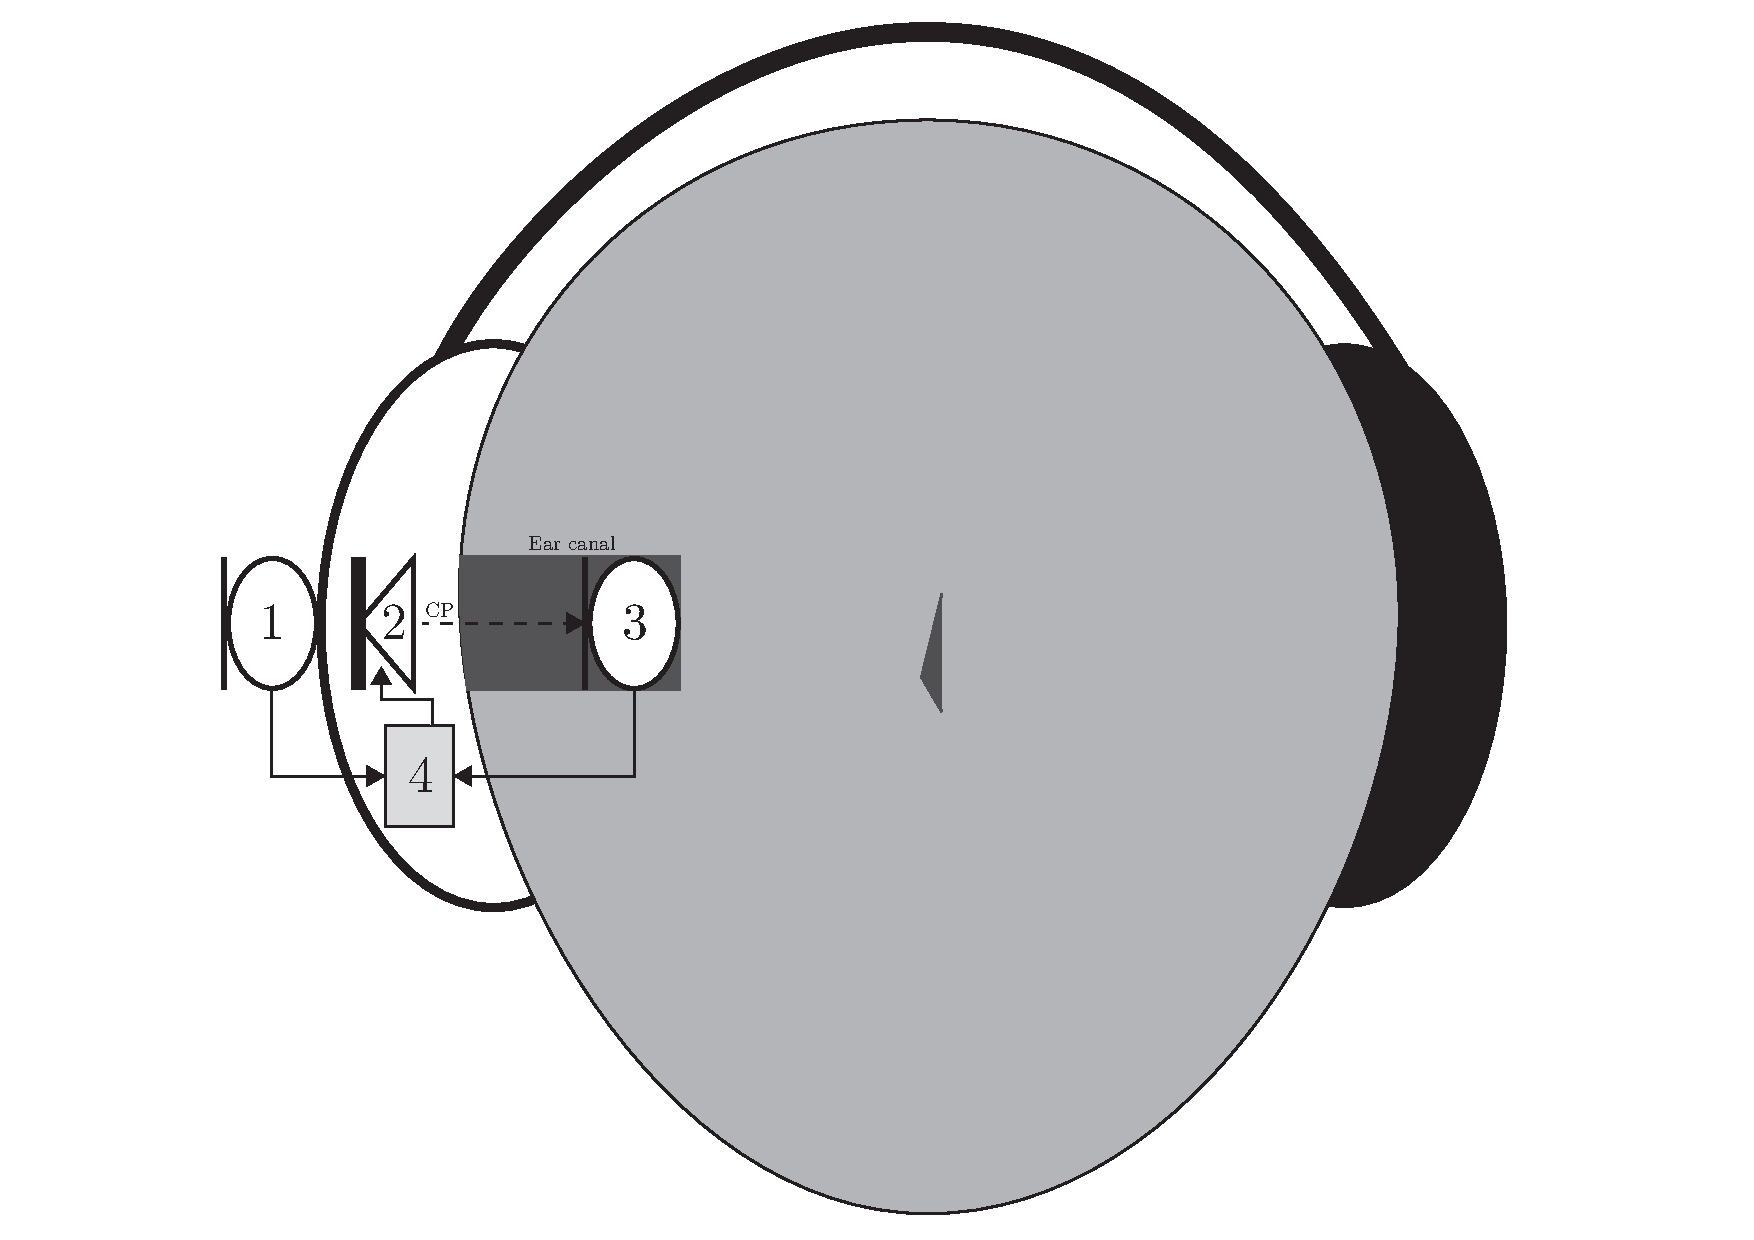
\includegraphics[width=3cm]{figures/BasicOverview}};

\draw  (3.14,1.65) rectangle (2.14,0.95);

\draw (1.56,1.31) -- (2.14,1.31);
\draw  (1.56,2.32) rectangle (-3.7,0.32);
\draw  (-5,-1.75) rectangle node[text width=2cm,align=center] {ADC \& Antialiasing filter} (-2.86,-3.25);
\draw  (-5,-6) rectangle node[text width=2.5cm,align=center] {Cancellation \\ path}(-2.75,-7.5);
\draw  (-1.23,-6) rectangle node[text width=2.5cm,align=center] {Adaptive FXLMS Algorithm} (1.27,-7.5);

\draw  (-3.45,-3.79) rectangle node[text width=1.5cm,align=center,fill=white] {Control filter} (-1.58,-5.29);
\draw  (-2.08,-1.75) rectangle node[text width=2.5cm,align=center] {DAC \& \\ Reconstruction filter}(0.37,-3.25);
\draw  (0.77,-1.75) rectangle node[text width=2cm,align=center] {ADC \& Antialiasing filter}(2.91,-3.25);

\draw  (-5.71,-0.69) rectangle (3.55,-7.76);
\node at (-5.06,-0.99) {DSP(4)};
\node [text width=2cm,align=center] at (-3.15,-1.2) {Reference Signal};

\draw[->] (-2.75,-7) -- node[above]{$f[n]$} (-1.23,-7);

\draw[->] (2.27,-3.25) -- node[right]{$e[n]$} (2.27,-7)  -- (1.27,-7);



\draw [->](-4,-3.25) -- (-4,-6);

\draw [->](-4,-4.79) node[left]{$x[n]$} -- (-3.45,-4.79);

\draw[->] (-1.58,-4.79) -- (-1.08,-4.79) --node[right]{$y[n]$} (-1.08,-3.25);

\node [text width=2cm,align=center] at (-0.38,-1.25) {Control Signal};
\node [text width=1.5cm,align=center] at (2.82,-1.25) {Error Signal};

\draw (-1.23,-6.4) -- (-1.83,-6.4) --node[above=3.25,right]{$\bar{b}[n+1]$} (-2.43,-5.29);
\draw [->](-3.1,-3.79) -- (-3.3,-3.43);


\draw[->] (0.48,1.06) -- (0.48,0) -- (2,0) -- (2,-1.76);
\draw[->] (-3.4,1.06) -- (-3.4,-0.16) -- (-4.2,-0.16) -- (-4.2,-1.76);
\end{tikzpicture}
		}
		\end{column}
	\end{columns}
\end{frame}


\subsection{Optimization}
\begin{frame}{Filtered-$x$ Least mean squares}{A minimization problem}
	\begin{columns}
		\begin{column}{0.5\textwidth}		
			
			\begin{itemize}
				\item Feedforward
				\begin{itemize}
					\item Dependent on delay between actuator and source		
				\end{itemize}
				\item Combined with an error microphone for feedback
				\begin{itemize}
					\item Adapt to changes in environment
					\item Always behind in samples/time 		
					\begin{itemize}
						\item Efficient for periodic signals
						\item Inefficient for stochastic signal 
					\end{itemize}	
				\end{itemize}
				\item Assumptions:
				\begin{itemize}
					\item Stationary Cancellation path
					\item FIR filter
				\end{itemize}
				
			\end{itemize}
			
			
		\end{column}
		\begin{column}{0.5\textwidth}
			\resizebox{0.85\columnwidth}{!}{	
			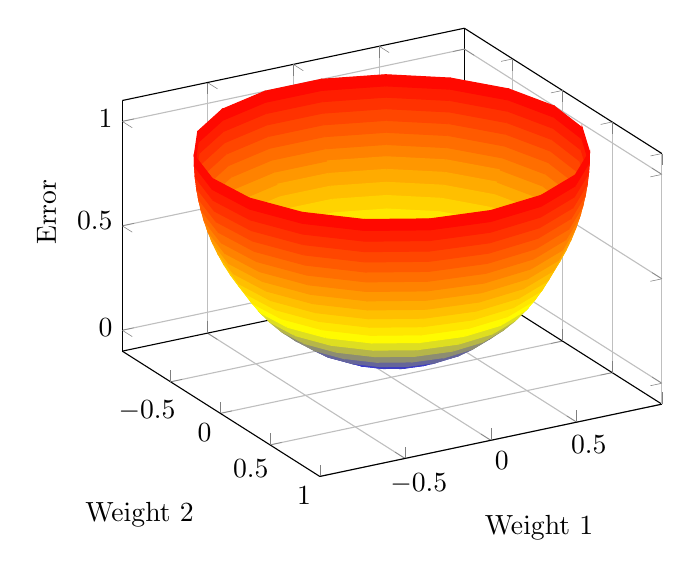
\begin{tikzpicture}
			\begin{axis}[
			view={60}{30},
			ylabel = {Weight 1},
			xlabel = {Weight 2},
			zlabel = {Error},
			zticklabels={1,0.5,0},ztick={0,-0.5,-1},
			grid=major,
			]
			\addplot3[surf,shader=flat,
			samples=20,
			domain=-1:0,y domain=0:2*pi,
			z buffer=sort]
			({sqrt(1-x^2) * cos(deg(y))},
			{sqrt( 1-x^2 ) * sin(deg(y))},
			x);	
			\end{axis}
			\end{tikzpicture}
			}
		\end{column}
	\end{columns}
\end{frame}


\subsection{Feedforward system}
\begin{frame}{Filtered-x Least mean square}{Adaptive FXLMS Algorithm}

	\begin{columns}
		\begin{column}{0.5\textwidth}
		\begin{center}
		

		\begin{itemize}
		\item[] Starting point:
		\begin{itemize}
		\setlength{\itemindent}{4em}
		\item[Input] $x[n]$
		\item[Output]$y[n]$
		\item[Error] $e[n]$	
		\item[Filtered x] $f[n]$	
		\item[Cancellation Path] $c[n]$		
		\end{itemize}

		\item[] Error Source:
		\begin{itemize}
		\item[] $e[n]=y[n]+x[n]$
		\end{itemize}

		\item[] Determining the gradient
		\begin{itemize}
		\item[] $\Delta b[n]=\frac{\partial e^2[n]}{\partial b[n]}=2e[n] \cdot \frac{\partial s[n]}{\partial b[n]}$
		\end{itemize}

		\item[] Utilizing the Filtered-x
		\begin{itemize}
		\item[] $\frac{\partial s[n]}{\partial b[n]} = [b_j[n] * x[n]]* c[n]$
		\end{itemize}		
		
		\item[] LMS expression:
		\begin{itemize}
		\item[] $b_j[n+1]=b_j[n]-2\mu e[n] f[n-j]$	
		\end{itemize}
		
		\end{itemize}
		\end{center}	
		
		
		
		
		\end{column}
		\begin{column}{0.5\textwidth}
		\resizebox{1.1\columnwidth}{!}{	
		\begin{tikzpicture}
\draw [](-2.92,2.32) node (v1) {} .. controls (-3.26,2.06) and (-3.26,0.54) .. (-2.92,0.32) node (v2) {};

\draw [draw=black,fill=black!20](-0.68,2.32) node (v1) {} .. controls (-1.08,2.06) and (-1.08,0.54) .. (-0.68,0.32) node (v2) {};
\draw [white, fill=black!20](-0.68,2.32) -- (1.56,2.32) -- (1.56,0.32) -- (-0.68,0.32);


\draw [draw=black,fill=black!60](-0.93,1.78) node (v1) {} .. controls (-0.99,1.59) and (-0.99,1.14) .. (-0.95,0.94) node (v2) {};
\draw [draw=black,fill=black!60](-0.93,1.78) -- (0.72,1.78) -- (0.72,0.94) -- (-0.95,0.94);


\draw [draw=black,fill=white] (0.48,1.36) node (v3) {3} ellipse (0.2 and 0.3);
\draw [draw=black,fill=black](0.28,1.66) -- (0.28,1.06);

\draw [draw=black,fill=white] (-3.4,1.36) node (v3) {1} ellipse (0.2 and 0.3);
\draw [draw=black,fill=black](-3.6,1.7) -- (-3.6,1.06);


\draw [draw=black,fill=black] (-2.9,1.7) rectangle (-3,1);
\draw (-2.9,1.3) -- (-2.6,1.7) -- (-2.6,1) -- (-2.9,1.3);
\node at (-2.7,1.34) {\small{2}};
\node at (-1.7,1.54) {\small{c[n]}};

\draw[->,dashed] (-2.6,1.36) node[right=0.5,above]{\small{}}-- (0.28,1.36);



\draw [->](-1.14,-1.76) -- (-1.14,-0.2) -- (-2.94,-0.2) -- (-2.94,1);
\node at (0,2) {\small{Ear Canal}};
\node[anchor=south west,inner sep=0] at (1.9,0.3) {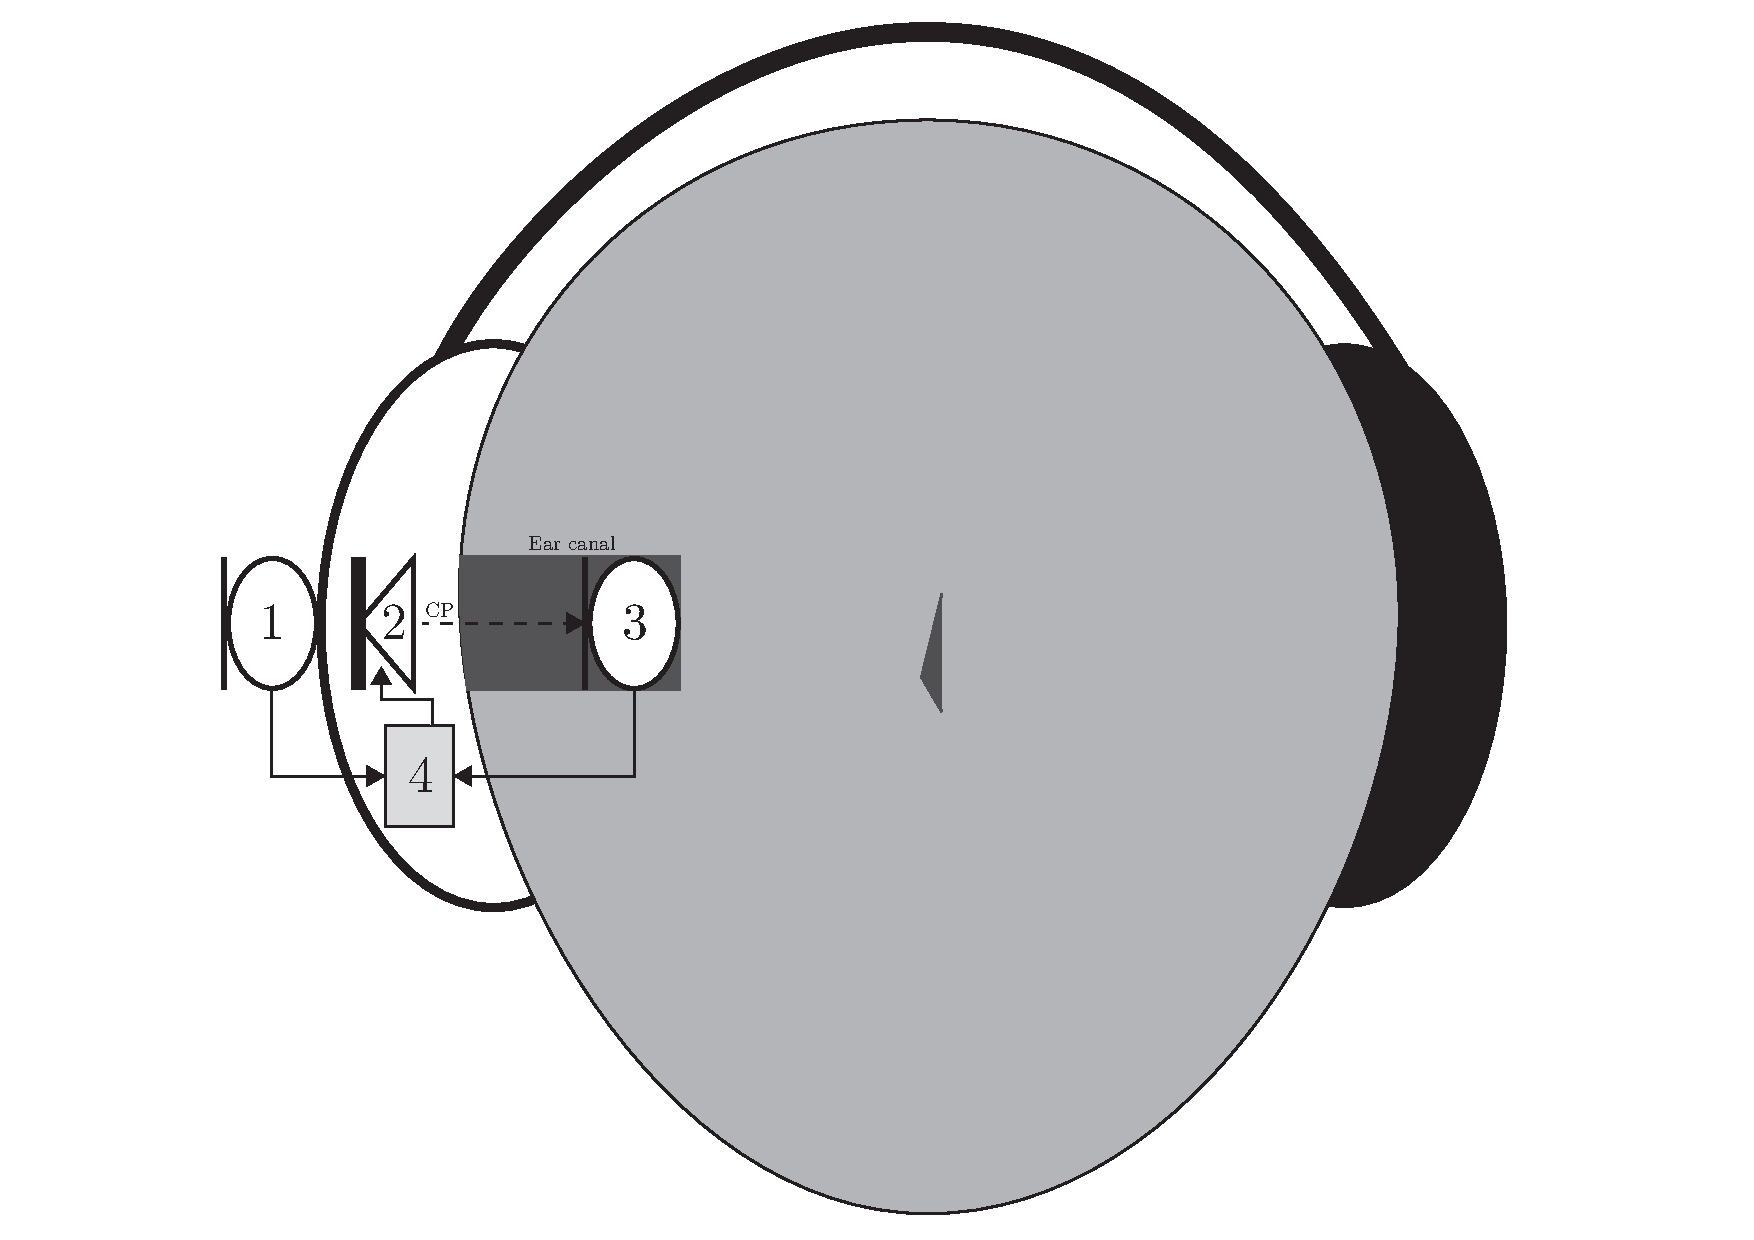
\includegraphics[width=3cm]{figures/BasicOverview}};

\draw  (3.14,1.65) rectangle (2.14,0.95);

\draw (1.56,1.31) -- (2.14,1.31);
\draw  (1.56,2.32) rectangle (-3.7,0.32);
\draw  (-5,-1.75) rectangle node[text width=2cm,align=center] {ADC \& Antialiasing filter} (-2.86,-3.25);
\draw  (-5,-6) rectangle node[text width=2.5cm,align=center] {Cancellation \\ path}(-2.75,-7.5);
\draw  (-1.23,-6) rectangle node[text width=2.5cm,align=center] {Adaptive FXLMS Algorithm} (1.27,-7.5);

\draw  (-3.45,-3.79) rectangle node[text width=1.5cm,align=center,fill=white] {Control filter} (-1.58,-5.29);
\draw  (-2.08,-1.75) rectangle node[text width=2.5cm,align=center] {DAC \& \\ Reconstruction filter}(0.37,-3.25);
\draw  (0.77,-1.75) rectangle node[text width=2cm,align=center] {ADC \& Antialiasing filter}(2.91,-3.25);

\draw  (-5.71,-0.69) rectangle (3.55,-7.76);
\node at (-5.06,-0.99) {DSP(4)};
\node [text width=2cm,align=center] at (-3.15,-1.2) {Reference Signal};

\draw[->] (-2.75,-7) -- node[above]{$f[n]$} (-1.23,-7);

\draw[->] (2.27,-3.25) -- node[right]{$e[n]$} (2.27,-7)  -- (1.27,-7);



\draw [->](-4,-3.25) -- (-4,-6);

\draw [->](-4,-4.79) node[left]{$x[n]$} -- (-3.45,-4.79);

\draw[->] (-1.58,-4.79) -- (-1.08,-4.79) --node[right]{$y[n]$} (-1.08,-3.25);

\node [text width=2cm,align=center] at (-0.38,-1.25) {Control Signal};
\node [text width=1.5cm,align=center] at (2.82,-1.25) {Error Signal};

\draw (-1.23,-6.4) -- (-1.83,-6.4) --node[above=3.25,right]{$\bar{b}[n+1]$} (-2.43,-5.29);
\draw [->](-3.1,-3.79) -- (-3.3,-3.43);


\draw[->] (0.48,1.06) -- (0.48,0) -- (2,0) -- (2,-1.76);
\draw[->] (-3.4,1.06) -- (-3.4,-0.16) -- (-4.2,-0.16) -- (-4.2,-1.76);
\end{tikzpicture}
		}
		\end{column}
	\end{columns}


\end{frame}

\section{Combined system}
\begin{frame}{Overview}{Combined System}	
	\begin{itemize}
		\item Input for control filter and CP
		\begin{itemize}
			\item $x[n]$
			\item $\hat{x}[n+P]$
		\end{itemize}
	\end{itemize}
	\begin{center}
		\resizebox{0.9\columnwidth}{!}{		
			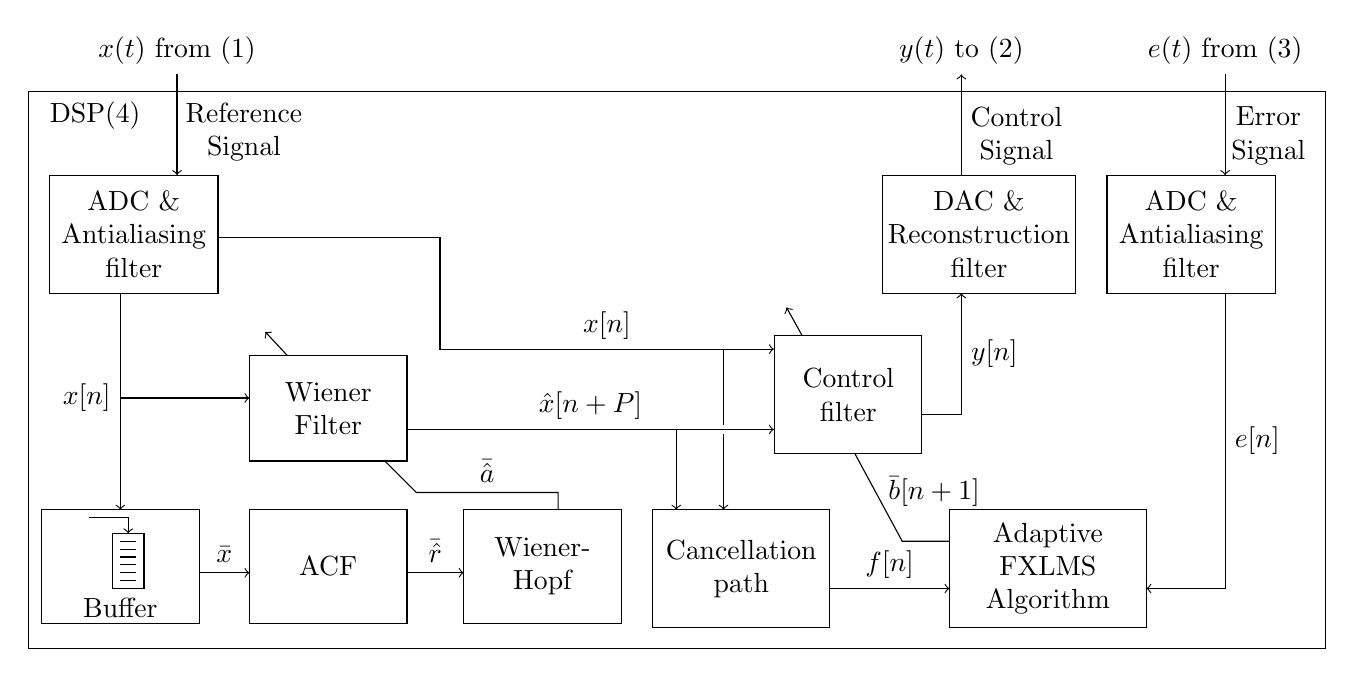
\begin{tikzpicture}
\draw  (-6.96,-2.17) rectangle node[text width=2cm,align=center] {ADC \& Antialiasing filter} (-4.82,-3.67);
\draw  (0.7,-6.42) rectangle node[text width=2.5cm,align=center] {Cancellation \\ path}(2.95,-7.92);
\draw  (4.47,-6.42) rectangle node[text width=2.5cm,align=center] {Adaptive FXLMS Algorithm} (6.97,-7.92);

\draw  (2.25,-4.21) rectangle node[text width=1.5cm,align=center,fill=white] {Control filter} (4.12,-5.71);
\draw  (3.62,-2.17) rectangle node[text width=2.5cm,align=center] {DAC \& \\ Reconstruction filter}(6.07,-3.67);
\draw  (6.47,-2.17) rectangle node[text width=2cm,align=center] {ADC \& Antialiasing filter}(8.61,-3.67);

\draw  (-7.23,-1.11) rectangle (9.25,-8.18);
\node at (-6.38,-1.41) {DSP(4)};
\node [text width=2cm,align=center] at (-4.49,-1.62) {Reference Signal};

\draw[->] (2.95,-7.42) -- node[above]{$f[n]$} (4.47,-7.42);

\draw[->] (7.97,-3.67) -- node[right]{$e[n]$} (7.97,-7.42)  -- (6.97,-7.42);

\draw [->](7.97,-0.89) node[above]{$e(t)$ from (3)} -- (7.97,-2.17) ;
\draw [->](4.62,-2.17)  --  (4.62,-0.89) node[above]{$y(t)$ to (2)};




\draw[->] (4.12,-5.21) -- (4.62,-5.21) --node[right]{$y[n]$} (4.62,-3.67);
\draw [->](-5.34,-0.89) node[above]{$x(t)$ from (1)} -- (-5.34,-2.17);
\node [text width=2cm,align=center] at (5.32,-1.67) {Control Signal};
\node [text width=1.5cm,align=center] at (8.52,-1.67) {Error Signal};

\draw (4.47,-6.82) -- (3.87,-6.82) --node[above=2.25,right]{$\bar{b}[n+1]$} (3.27,-5.71);
\draw [->](2.6,-4.21) -- (2.4,-3.85);


%% Boxes
\draw  (-4.42,-5.8) rectangle node[text width=2cm,align=center] {Wiener Filter}(-2.42,-4.46);
\draw  (-2.42,-6.42) rectangle node[text width=2cm,align=center] {ACF}(-4.42,-7.86);
\draw  (-5.06,-6.42) rectangle node[text width=2cm,align=center,below=8] {Buffer}(-7.06,-7.86);
\draw  (-1.7,-6.42) rectangle node[text width=1.5cm,align=center] {Wiener- Hopf}(0.3,-7.86);



%%Buffer
\draw (-5.76,-7.42) node (v1) {} -- (-6.16,-7.42) -- (-6.16,-6.72) -- (-5.76,-6.72) -- (-5.76,-7.42);
\draw (-6.06,-6.82) -- (-5.86,-6.82);
\draw (-6.06,-6.92) -- (-5.86,-6.92);
\draw (-6.06,-7.02) -- (-5.86,-7.02);
\draw (-6.06,-7.12) -- (-5.86,-7.12);
\draw (-6.06,-7.22) -- (-5.86,-7.22);
\draw (-6.06,-7.32) -- (-5.86,-7.32);
\draw [->](-6.46,-6.52) -- (-5.96,-6.52) -- (-5.96,-6.72);


%% Lines
\draw [->](-5.06,-7.22) -- node[above]{$\bar{x}$} (-4.42,-7.22);
\draw [->](-2.42,-7.22) -- node[above]{$\bar{\hat{r}}$}(-1.7,-7.22);
\draw (-0.5,-6.42) -- (-0.5,-6.2) -- node[above]{$\bar{\hat{a}}$} (-2.3,-6.2) -- (-2.7,-5.8);


\draw [->](-3.94,-4.46) -- (-4.22,-4.16);
\draw [->](-6.06,-5)  node[left]{$x[n]$} -- (-4.42,-5);
\draw [->](-6.06,-3.68) -- (-6.06,-6.42);
\draw [->](-2.42,-5.4) --  node[above]{$\hat{x}[n+P]$}(2.24,-5.4);

\draw [->](-4.82,-2.96) -- (-4.56,-2.96) -- (-2,-2.96) -- (-2,-4.38) -- node[above]{$x[n]$} (2.24,-4.38);
\draw (1.6,-4.38) -- (1.6,-5.34);
\draw [->](1.6,-5.46) -- (1.6,-6.42);
\draw [->](1,-5.4) -- (1,-6.42);
\end{tikzpicture}}
	\end{center}
\end{frame}


\subsection{Multirate}
\begin{frame}{Implementation Consideration}{Multirate}

	\begin{columns}
		\begin{column}{0.4\textwidth}
\begin{itemize}
\item Reduce to computation demands N-fold

\begin{itemize}
\item Lower prediction length
\item 12 kHz is a factor $2^4$ lower in computation cost 
\end{itemize}
\end{itemize}
		\end{column}
		\begin{column}{0.6\textwidth} 
		
		\begin{center}
\begin{table}[]
\centering
\begin{tabular}{|c|c|c|c|c|c|}
\hline
$fs$                                                          & 192 & 96 & 48 & 24 & 12 \\ \hline
\begin{tabular}[c]{@{}c@{}}Prediction\\ Length\end{tabular}   & 43  & 22 & 11 & 6  & 3  \\ \hline
\end{tabular}
\end{table}
		\resizebox{0.75\columnwidth}{!}{
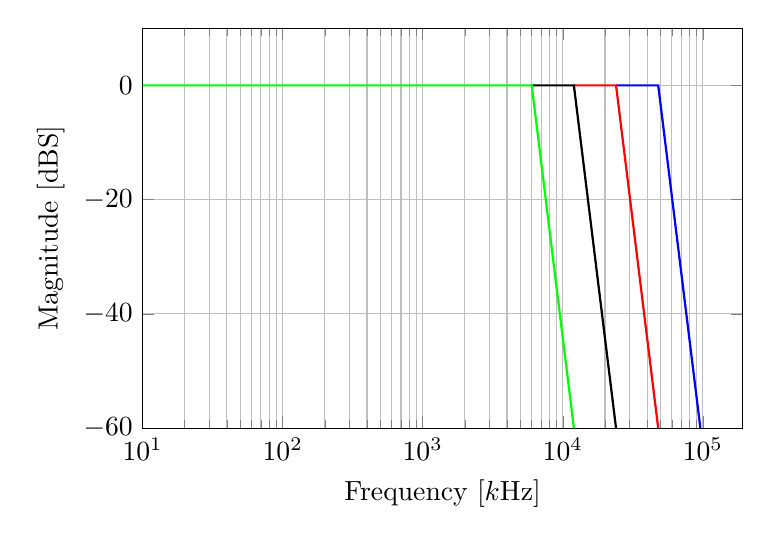
\begin{tikzpicture}
\begin{axis}[
width=3in,
height=2in,
scale only axis,
unbounded coords=jump,
xmode=log,
xmin=10,
xmax=192000,
xminorticks=true,
xlabel={Frequency [$k$Hz]},
xmajorgrids,
xminorgrids,
ymin=-60,
ymax=10,
ylabel={Magnitude [dBS]},
ymajorgrids,
axis background/.style={fill=white},
]
\addplot[mark=none, blue,thick] coordinates {(24000,0) (48000,0) (96000,-60)};
\addplot[mark=none, red,thick] coordinates {(12000,0) (24000,0) (48000,-60)};
\addplot[mark=none, black,thick] coordinates {(6000,0) (12000,0) (24000,-60)};
\addplot[mark=none, green,thick] coordinates {(10,0) (6000,0) (12000,-60)};
\end{axis}
\end{tikzpicture}
}
		\end{center}	
		\end{column}
	\end{columns}
\end{frame}
